Figure \ref{fig:workflow-glai-time-series} shows the proposed workflow. Based on in-situ \gls{GLAI} (\textit{"in-situ GLAI"}) values and air temperature data at the calibration sites (Section \ref{subsec:calibration-data}), \gls{DRC}s are fitted and used to model growth rates in hourly and daily resolution (Figure~\ref{fig:workflow-glai-time-series}a). \gls{S2} \gls{GLAI} (\textit{"raw GLAI"}) observations at the validation sites (Section \ref{subsec:validation-data}, Figure \ref{fig:workflow-glai-time-series}b) are assimilated into the \gls{DRC}-based growth curves and used to reconstruct the \gls{GLAI} time series (\textit{"DRC GLAI"}) (Figure \ref{fig:workflow-glai-time-series}c). In addition, a baseline is fit based solely on \gls{S2} \gls{GLAI} observations (\textit{"baseline GLAI"}) using a sigmoid function (Figure \ref{fig:workflow-glai-time-series}d). In a last step, the reconstructed \gls{GLAI} time series are compared to in-situ validation data. The term "coarse spatial resolution", as depicted in Figure \ref{fig:workflow-glai-time-series}, indicates that the meteorological data offered only one reading for each field parcel, without accounting for any within-field variability. On the other hand, high spatial resolution implies that the spatial intricacies regarding within-field heterogeneity are taken into account. Code and data necessary to reproduce all processing and analysis are available under GNU General Public License v3.0\footnote{\url{https://github.com/EOA-team/sentinel2_crop_trait_timeseries}}. The methods section follows this structure and starts with the processing of the in-situ data.

\begin{figure}[H]
    \centering
    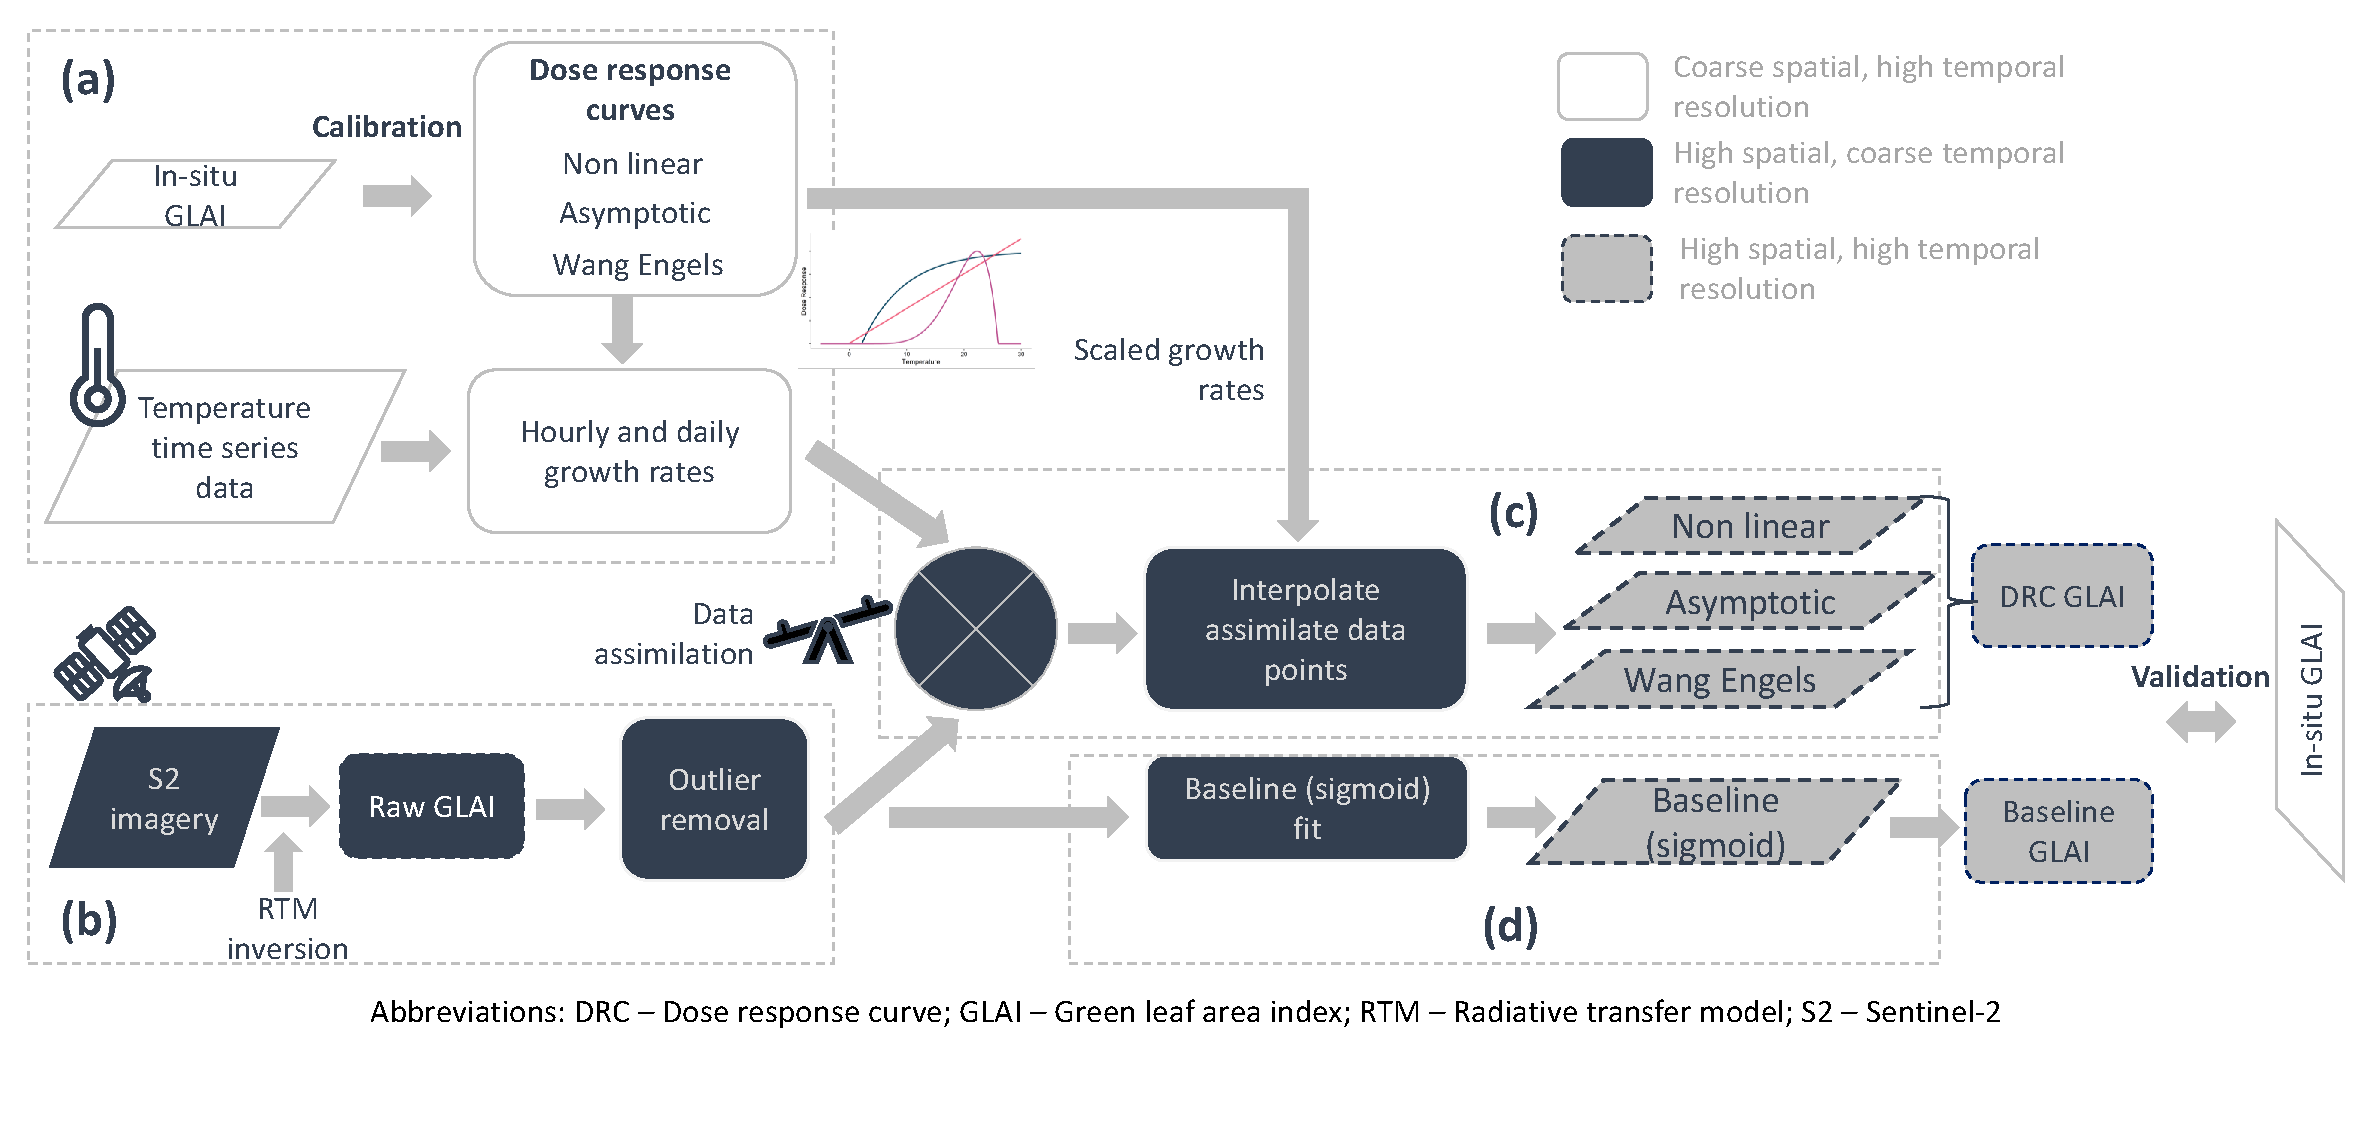
\includegraphics[width=1.0\textwidth]{06-DRC/img/workflow_glai_ts_reconstruction.pdf}
    \caption{Proposed workflow to reconstruct continuous \gls{GLAI} time series with high spatial and temporal resolution using temperature-based \gls{DRC}s to obtain \gls{GLAI} growth rates (a), \gls{S2} raw \gls{GLAI} observations per pixel (b) and data assimilation and \gls{DRC}-based interpolation of assimilated \gls{DRC} \gls{GLAI} values (c). The baseline method using a sigmoid function fit to the \gls{S2} \gls{GLAI} data (baseline \gls{GLAI}) is shown in (d).}
    \label{fig:workflow-glai-time-series}
\end{figure}

\subsection{Processing of in-situ data}
Throughout the main growing season of winter wheat (beginning of March till end of June in central Europe) continuous, mostly weekly measurements of \gls{GLAI} and phenology were undertaken at the calibration (Section~\ref{subsec:calibration-data}) and validation sites (Section~\ref{subsec:validation-data}). All measurements were linked to hourly air temperature readings 2 m above ground available from nearby weather stations.

\subsubsection{Air temperature data}
Air temperature data was acquired hourly 2 m above ground in deg C. In addition, the temperature readings were aggregated to daily resolution by averaging all 24 hourly measurements of a day from midnight to midnight.

\subsubsection{Green Leaf Area Index}
\label{subsubsec:glai-processing}
\gls{GLAI} samples were derived non-destructively using a LAI-2200C Plant Canopy Analyzer by LI-COR Biosciences with a 45 degree viewing cap. Measurements were performed at pre-defined sampling points within the fields (see, e.g., Figure~\ref{fig:map-validation-sites}a). For each measurement, three replicates were performed in different orientations each of them offset by 90 degrees. To avoid contamination of the measurement by direct sun light the measurements were either shaded manually, taken under diffuse light conditions (over-cast sky, fog) or acquired early in the morning.

\subsubsection{Phenology}
\label{subsubsec:phenology-processing}
Estimates of \gls{GLAI} (Section~\ref{subsubsec:glai-processing}) were linked to phenological development.
Phenological development of the winter wheat canopies was expressed in \gls{BBCH} scale following~\cite{lancashire_uniform_1991}. For the rating of the beginning of stem elongation (BBCH 30) we cut the main tiller lengthwise and measured the distance between the first node and the tillering node following the manual by~\cite{pask_physiological_2012}. End of heading (BBCH 59) was reached when the inflorescence was fully emerged.

\subsection{Model calibration to introduce physiological knowledge}
\label{subsec:model-cal}

Model calibration introduces the a-priori physiological knowledge about the relationship between plant growth and air temperature (Figure \ref{fig:workflow-glai-time-series}a). The knowledge was based on a dataset of in-situ \gls{GLAI} measurements from the calibration sites (Section~\ref{subsec:calibration-data}). The measured in-situ \gls{GLAI} values were used to calculate \gls{deltaGLAI} between two time points, which represent increase, respectively growth of the wheat canopy (Equation~\ref{eq:delta_LAI}) (as in \cite{tschurr_frost_2023}). In-situ \gls{GLAI} values have been smoothed using cubic smoothing splines before the calculation of \gls{deltaGLAI}.

\begin{equation}
\label{eq:delta_LAI}
  \Delta GLAI(t_n) =  GLAI(t_{n}) - GLAI(t_{n-1})\,,
\end{equation}

The \gls{deltaGLAI} value can then be expressed using the temperature trajectory between time point t\textsubscript{n} and t\textsubscript{n-1} in either hourly or daily granularity.

\subsubsection{Fitting of Dose-Response Curves}
\label{subsubsec:fitting-drc}
% DRCs
The calibration dataset was utilised to optimise three distinct \gls{DRC}, as illustrated in Figure~\ref{fig:DRC_overview}. Each curve represents the behaviour of the \gls{deltaGLAI} as a function of the observed temperature. The simplest \gls{DRC} displays a non-linear correlation between growth and temperature, with zero growth deemed below $T_{base}$. A linear growth reaction is projected for temperatures exceeding $T_{base}$. We hereafter refer to this growth response curve as the non-linear DRC (e.g., as seen in \cite{roth_field_2023}). Additionally, an asymptotically shaped DRC was employed, accounting for a base temperature ($T_{base}$), below which no growth occurs. Above $T_{base}$, the DRC exhibits a maximum growth response, defined by the curve's asymptote, along with the parameter lrc, allowing for an asymptotic shape of the curve (e.g., see \cite{roth_phenomics_2022}). Similar to the asymptotic \gls{DRC}, the Wang Engels \gls{DRC} can be defined by three parameters: $T_{base}$, which is the temperature below which growth does not occur, $T_{opt}$, which defines the highest growth rate response, and $T_{max}$, which is the temperature above which the growth rate is set to zero~\citep{wang_simulation_1998, wang_uncertainty_2017} (refer to Figure~\ref{fig:DRC_overview}).

\begin{figure}[H]
    \centering
    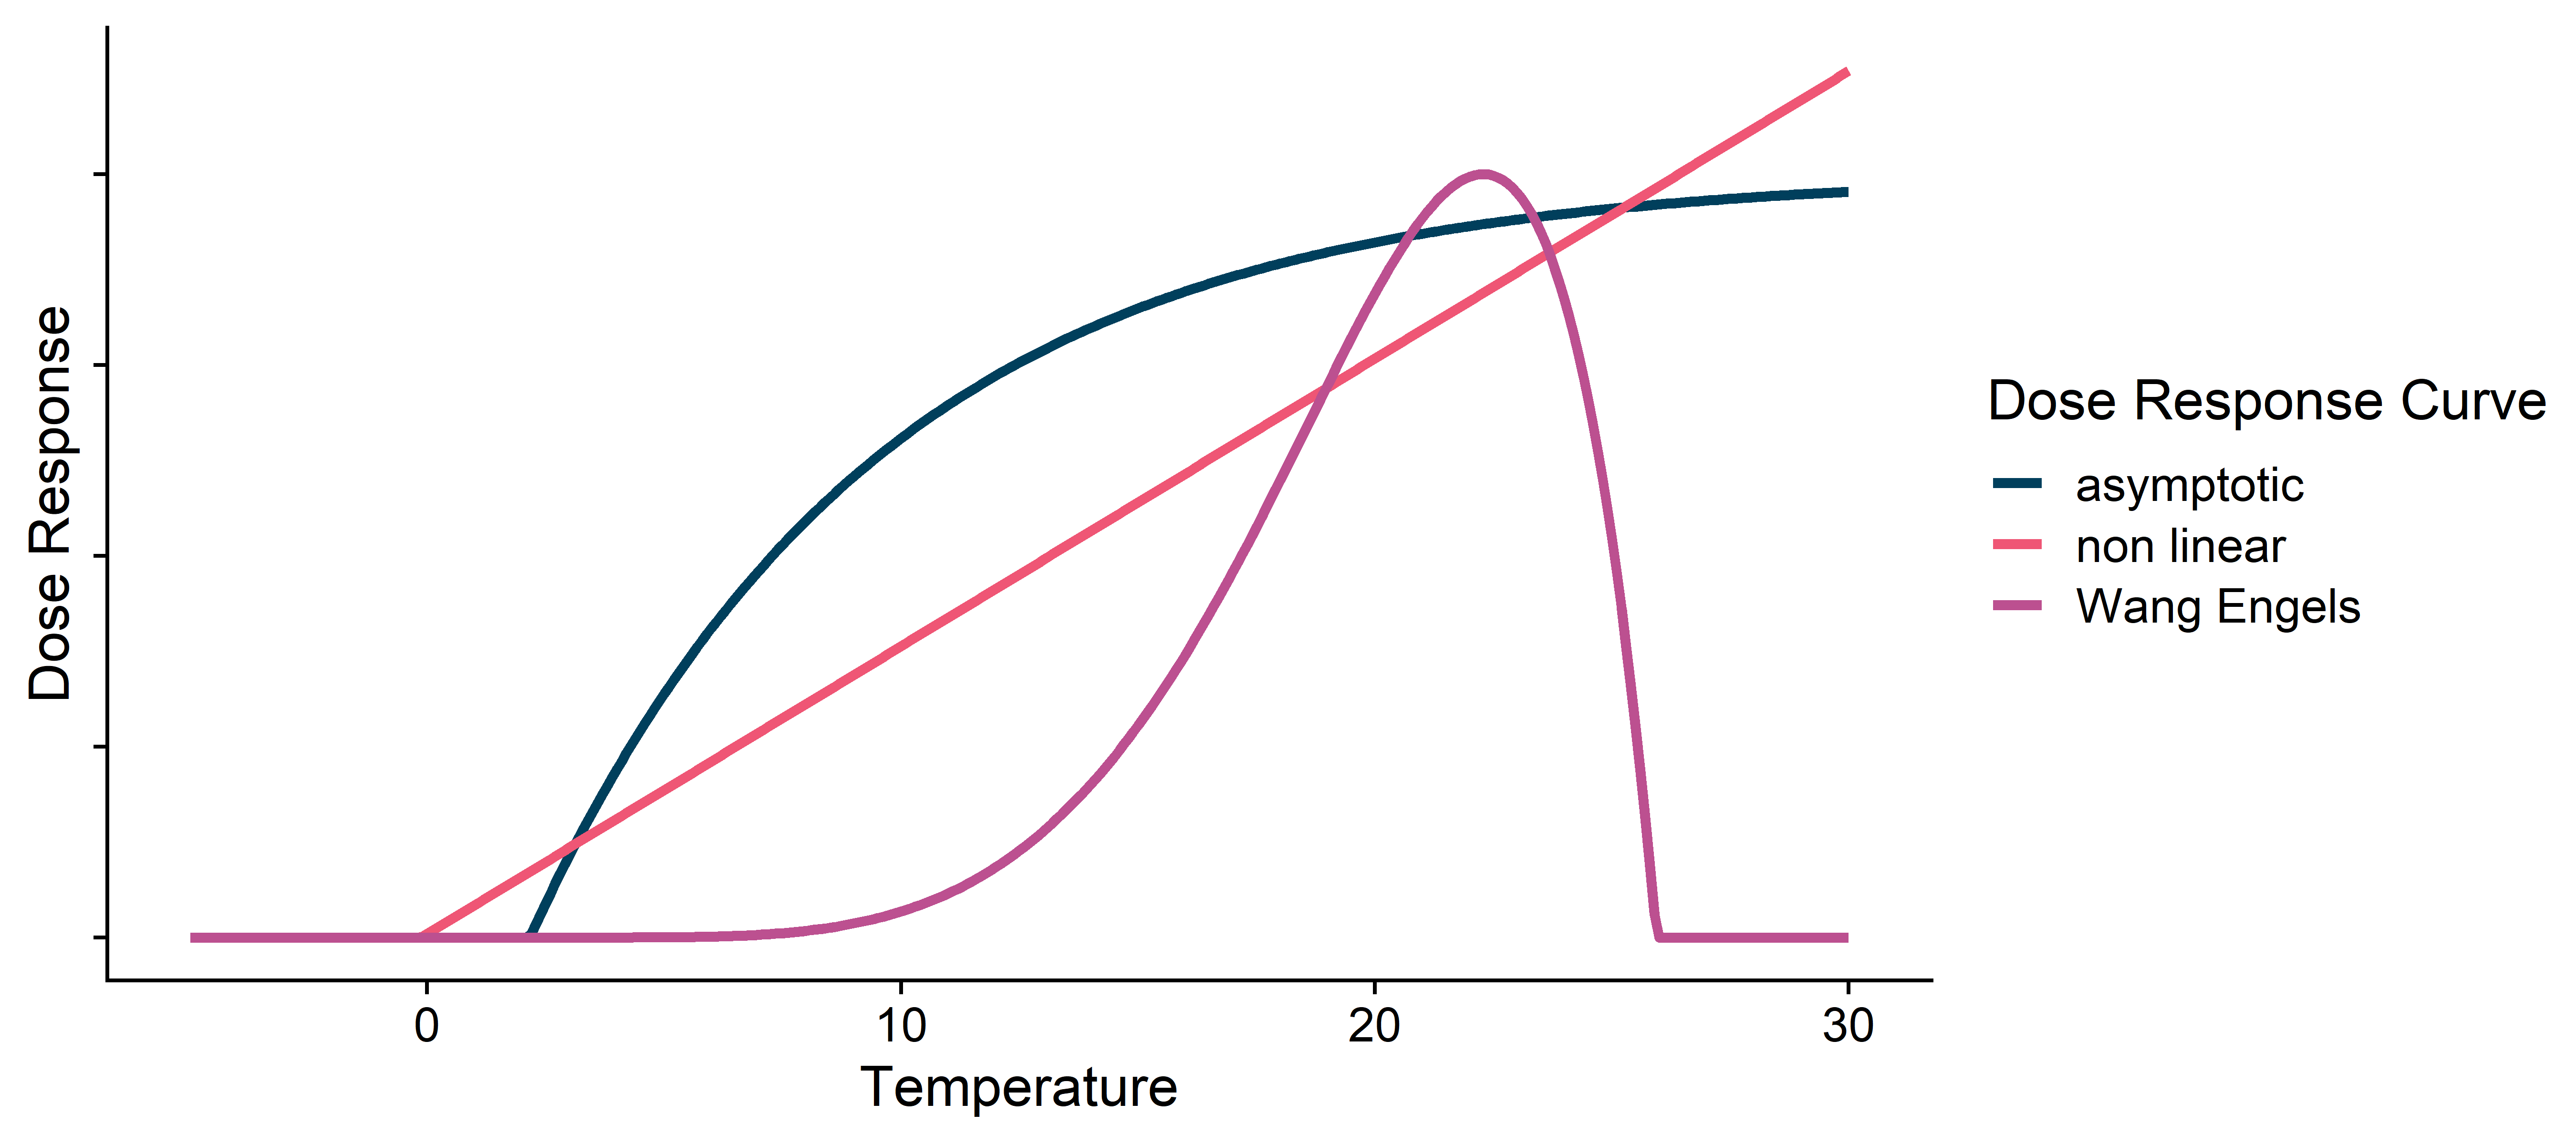
\includegraphics[width=0.8\textwidth]{06-DRC/img/DRC_curves_scheme.png}
    \caption{Schematic overview of the three used dose response curves (DRC), non linear, asymptotic and Wang Engels curve. The x axis represents the input temperature, the y axis the corresponding response in green leaf area index (GLAI) growth.}
    \label{fig:DRC_overview}
\end{figure}


\begin{table}[H]
\caption{Dose response curve parameters and constraints used for model fitting.}
\label{tab:drc_fitting}
\centering
\begin{tabular}{lll}
Dose response curve & parameters                       & constraints                          \\ \hline
non linear          & $T_{base}$ , slope         &                                      \\
asymptotic          & $T_{base}$, lrc, asymptote & $T_{base}$ \textless asymptote \\
Wang Engels &
  \begin{tabular}[c]{@{}l@{}} $T_{base}$,\\  $T_{opt}$,\\   $T_{max}$\end{tabular} &
  \begin{tabular}[c]{@{}l@{}} $T_{base}$\\  \textless $T_{opt}$ \\ \textless  $T_{max}$\end{tabular}
\end{tabular}
\end{table}

% fitting nloptr
The parameters for each of the three DRCs (refer to Table~\ref{tab:drc_fitting}) were optimised utilising the calibration data explained earlier. An augmented Lagrangian algorithm employing the nloptr package in R \citep{rcore-team_r_2014,johnson_nlopt_2007} was used for this purpose. Regarding our third research question, optimisation was conducted for temperature values of both hourly and daily measurements.

As the curves used can solely depict ascending \gls{GLAI} values, we excluded negative \gls{deltaGLAI} values prior to optimization. These values are typically attributable to measurement uncertainty and imprecisions, such as those related to sensor positioning. As a result, 20\% of \gls{deltaGLAI} values were rejected. Constrained optimization by linear approximation (COBYLA) was used as the local solver for optimization, providing upper and lower bounds and a starting value \citep{powell_direct_1994}. Initial values were determined either by quantile values of input temperature data (for $T_{base}$, $T_{opt}$, and $T_{max}$) or by empirically derived values (slope, lrc, and asymptote) (refer to Table \ref{tab:Sup_starting_paramters} in the Appendix). Optimisation was carried out 20 times on a randomly selected 80\% of the data, and the final parameters were derived from the median of the 20 subset optimisations to obtain more robust parameter values, thereby reducing the possible influence of outliers. For each temperature measurement, the corresponding dose response value was calculated and accumulated over time. To optimise the parameters, the \gls{RMSE} between these accumulated values and the \gls{deltaGLAI} measurements was minimised. The skill score was negatively impacted for meeting constraints (Table~\ref{tab:drc_fitting}) or for forecasting \gls{deltaGLAI} values that were too low to attain physiologically significant parameter and prediction values.

\subsection{Processing of \gls{S2} data}

\gls{S2} raw \gls{GLAI} observations introduce spatial detail (Figure \ref{fig:workflow-glai-time-series}b).
We used all 10 and 20 m bands except band 8 (central wavelength 842 nm). Band 8 was discarded in favor of band 8A (central wavelength 865 nm) which provides a higher spectral resolution than band 8. Thus, nine bands between 492 and 2200 nm were used: B2 (blue), B3 (green), B4 (red), B5 (red-edge 1), B6 (red-edge 2), B7 (red-edge 3), B8A (near-infrared 2), B11 (shortwave-infrared 1), and B12 (shortwave-infrared 2). See also Table \ref{tab:s2-bands} in the Appendix for details about the native spatial resolution, spectral band widths and central wavelengths of these bands.

First, we clipped the \gls{S2} data to the spatial extent of the field parcels at the validation sites (Figure~\ref{fig:map-validation-sites}a). Next, we resampled the six 20 m bands (see Table \ref{tab:s2-bands}) to a spatial resolution of 10 m using nearest neighbor interpolation.

All scenes were pre-processed by ESA using the payload data ground segment (PDGS) baselines 4.00 (2022 data) and 5.09 (2023 data) that compromise an improvement radiometric harmonization of S2A and S2B as well as geometric refinements that fulfil the CEOS Analysis Ready Data for Land (CEOS ARD) standard. Therefore, no further refinements such as image co-registration were undertaken.

\subsubsection{Data cleaning}
We used the \gls{SCL} delivered as part of the \gls{S2} L2A product to filter out clouds, shadows, open water, snow and cirrus on a per-pixel basis. Thus, only the SCL classes 4 (vegetation) and 5 (bare soil) were kept. Pixel values with a different \gls{SCL} class assignment were masked and not considered any further.

\subsubsection{Radiative transfer modelling}
To extract raw \gls{GLAI} from \gls{S2} scenes at the validation sites (Section~\ref{subsec:s2-imagery}) we used the four-stream \gls{RTM} PROSAIL~\citep{jacquemoud_prospectsail_2009} to simulate bi-directional reflectance factors of winter wheat canopies. PROSAIL couples the leaf \gls{RTM} PROSPECT-D~\citep{feret_prospect-d_2017} with the canopy \gls{RTM} 4SAIL~\citep{verhoef_light_1984}. We parameterized the \gls{RTM} inputs to reflect typical physiological and morphological characteristics of winter wheat canopies between \gls{BBCH} stages 30 and 59 based on a comprehensive field phenotyping dataset described in \cite{graf_insights_2023}. The leaf (PROSPECT-D) and canopy (4SAIL) input parameters including their range and distribution are shown in Table~\ref{tab:drc-prosail-inputs} based on \cite{graf_insights_2023}. Following the proposed workflow by \cite{graf_insights_2023} we increased the physiological plausibility of \gls{RTM} inputs. In detail, the leaf chlorophyll a+b and leaf carotenoid content were re-distributed based on empirical relationships between these traits and the \gls{GLAI} established in \cite{graf_insights_2023} (GLAI - Cab relationship) and \cite{wocher_rtm-based_2020} (Cab - Car relationship). Using these relationships we can re-distribute Cab (through the canopy chlorophyll content) solely based on \gls{GLAI}. Similarly, Car can be re-distributed solely based on Cab obtained in the previous step.

We run PROSAIL in forward mode based on the input parameters denoted in Table~\ref{tab:drc-prosail-inputs} for each \gls{S2} scene during the stem elongation period. Illumination and observer angles were set to scene-specific values obtained from the \gls{S2} scene metadata. In total, we run 50 000 PROSAIL simulations per \gls{S2} scene. The resulting spectra were converted to the spectral resolution of \gls{S2} by convolution of the original PROSAIL outputs in 1 nm spectral resolution with the spectral response functions of \gls{S2}A and B provided by ESA\footnote{\url{https://sentinel.esa.int/web/sentinel/user-guides/sentinel-2-msi/document-library/-/asset_publisher/Wk0TKajiISaR/content/sentinel-2a-spectral-responses}}. In addition, we applied further physiological plausibility checks introduced by~\cite{wocher_rtm-based_2020}. In detail, we dropped simulated spectra with a shift of the green reflectance peak towards wavelengths shorter than 574 nm, which was considered implausible based on extensive survey of handheld and airborne hyperspectral imaging data of green vegetation. Around 10\% of the simulated PROSAIL spectra were therefore discarded. The resulting spectra were stored in lookup tables (\gls{LUT}s) per \gls{S2} scene.

\begin{table}[H]
\caption{Parameter ranges and distributions for the combined leaf (PROSPECT-D) and canopy (4SAIL) \gls{RTM} (PROSAIL) for winter wheat canopies in the stem elongation phase. The ranges are given for uniform distributions (range) or a truncated Gaussian distribution with mean and standard deviation denoted in brackets. Cab and Car are redistributed on \gls{GLAI}. All values and distributions are taken from \cite{graf_insights_2023}.}
\label{tab:drc-prosail-inputs}
\begin{tabular}{@{}lllllll@{}}
\toprule
  \textbf{Trait}     & \textbf{Description}         & \textbf{Unit}           & \multicolumn{4}{l}{\textbf{Range}}              \\ \midrule
\multicolumn{7}{l}{\textbf{PROSPECT-D (Leaf)}}                                                                \\
\midrule
N      & Leaf Structure Parameter     & {[}-{]}                 & \multicolumn{4}{l}{1 - 2.5 (1.5, 0.2)}          \\
Cab    & Leaf Chlorophyll a+b Content & {[}$\mu g$ $cm^{-2}${]} & \multicolumn{4}{l}{redistributed based on GLAI} \\
Car    & Leaf Carotenoid Content      & {[}$\mu g$ $cm^{-2}${]} & \multicolumn{4}{l}{redistributed based on Cab}  \\
Cant   & Leaf Anthocyanin Content     & {[}$\mu g$ $cm^{-2}${]} & \multicolumn{4}{l}{0.0 - 5.0 (2.0, 0.8)}        \\
Cbrown & Brown Pigments               & {[}-{]}                 & \multicolumn{4}{l}{0 - 1}                       \\
Cw     & Equivalent Water Thickness   & {[}cm{]}                & \multicolumn{4}{l}{0 - 0.07 (0.04, 0.02)}       \\
Dm     & Dry Matter Content           & {[}$g$ $cm^{-2}${]}     & \multicolumn{4}{l}{0 - 0.01}                    \\
\midrule
\multicolumn{7}{l}{\textbf{4SAIL (Canopy)}}                                                                     \\
\midrule
GLAI   & Green Leaf Area Index        & {[}$m^2$ $m^{-2}${]}    & \multicolumn{4}{l}{0.5-6.5}                         \\
ALA    & Leaf Inclination Angle       & {[}deg{]}               & \multicolumn{4}{l}{30 - 70}                     \\
hspot  & Hot spot Parameter           & {[}-{]}                 & \multicolumn{4}{l}{0.01 - 0.5}                  \\
rsoil  & Soil Brightness Factor       & {[}-{]}                 & \multicolumn{4}{l}{0 - 1}                       \\
psoil  & Dry/ Wet Soil Factor         & {[}-{]}                 & \multicolumn{4}{l}{0 - 1}                       \\ \bottomrule
\end{tabular}
\end{table}


\subsubsection{Radiative transfer model inversion}
\label{subsubsec:rtm-inv}
For \gls{RTM} inversion we used the PROSAIL spectra stored in \gls{LUT}s per scene. We retrieved raw \gls{GLAI} per \gls{S2}  pixel by comparing \gls{S2}-observed ($\rho_{S2}$) spectra with the simulated spectra in the \gls{LUT} ($\rho_{LUT}$) by means of the \gls{MAE} for all $n$ \gls{S2}-bands considered (i.e., $n=9$) as suggested by \cite{graf_insights_2023}.

\begin{equation}
    MAE = \frac{1}{n} \sum_{i=0}^{n} |\rho_{{S2}_i} - \rho_{{LUT}_i} |
\end{equation}
The median \gls{GLAI} value obtained from the 5000 simulated spectra with the smallest \gls{MAE} was then used as the \gls{S2}-derived raw \gls{GLAI} observation per \gls{S2} pixel.


\subsection{Time series reconstruction}
\label{subsec:drc-model-inference}

\subsubsection{DRC-derived growth rates at the farm scale}

Fitted \gls{DRC}s were applied to hourly and daily air temperature data at the validation sites (Section~\ref{subsec:validation-data}, Figure \ref{fig:workflow-glai-time-series}a). This converted each air temperature reading into a \gls{GLAI} growth rate. Thus, per site and \gls{DRC} \gls{GLAI} growth rates in hourly and daily resolution were available.

\subsubsection{S2-derived raw GLAI observations at the pixel scale}
\label{subsubsec:s2-glai-simple-outlier-filter}
A simple outlier detection formalism was introduced to account for undetected atmospheric disturbances in the raw \gls{S2} \gls{GLAI} observations (Figure \ref{fig:workflow-glai-time-series}b). Atmospheric disturbances usually cause negatively biased outliers in remotely-sensed trait observations~\citep{chen_simple_2004}. Therefore, raw \gls{S2} \gls{GLAI} values of a pixel that deviated from the mean of all raw \gls{GLAI} values by more than a single standard deviation in the negative y-direction were discarded. This did not apply to the first \gls{GLAI} observation in time due to two reasons: First, we lack sufficient temporal context. Second, due to its proximity to the early phase of stem elongation a low \gls{GLAI} value is physiologically plausible.

\subsubsection{Data assimilation using Ensemble Kalman Filtering}
We aimed to combine the modelled \gls{DRC} \gls{GLAI} growth rates reflecting a-priori physiological knowledge about the relationship of growth to air temperature with raw \gls{S2} \gls{GLAI} observations to obtain the best possible estimate of the effective \gls{GLAI} (Figure \ref{fig:workflow-glai-time-series}c). Combining models with observations presents a data assimilation problem. In our case, we assimilated the raw \gls{S2} \gls{GLAI} observations into the \gls{DRC}-based \gls{GLAI} growth rates to introduce spatial detail while retaining the high temporal resolution and physiological meaning of the underlying temperature data.

For data assimilation, the \gls{KF} is widely used. In essence, \gls{KF} is a sequential approach estimating the "true", hidden state vector of a system by updating the modelled states whenever an observation becomes available. In our case, the hidden state vector is given by the actual but unknown \gls{GLAI} time series of a pixel. Since, both, the \gls{DRC} models and the \gls{S2} observations have uncertainties, we use the probabilistic \gls{EnsKF}. The \gls{EnsKF} allows to include model and observation uncertainty into the data assimilation process~\citep{evensen_ensemble_2003}. \gls{EnsKF} frameworks have therefore been widely used in assimilating remotely sensed crop traits in crop models~\citep{de_wit_crop_2007, zhao_assimilating_2013, huang_assimilating_2016}. ~\cite{graf_propagating_2023} found that raw \gls{GLAI} values derived from \gls{S2} take relative standard uncertainties up to 5\% due to uncertainty in the \gls{S2} top-of-atmosphere reflectance data. For in-situ \gls{GLAI} and temperature data we estimated a similar magnitude of uncertainty and set relative model uncertainty to 5\%. The \gls{EnsKF} ensemble size was set to 50 ensemble members to balance computational complexity with statistical significance as suggest by ~\cite{de_wit_crop_2007} and ~\cite{zhao_assimilating_2013}.

Figure~\ref{fig:assimilation-sample-pixel} shows the proposed data assimilation approach, i.e., a zoom-in into Figure~\ref{fig:assimilation-sample-pixel}c, for a randomly selected \gls{S2} pixel at the Strickhof site in 2022. Figure \ref{fig:assimilation-sample-pixel}a denotes the hourly air temperature time series available from the nearby weather station that was input into the \gls{DRC}s to obtain hourly \gls{GLAI} growth rates. The raw \gls{S2} \gls{GLAI} observations (red dots) were assimilated into the \gls{DRC} \gls{GLAI} growth rates (Figure \ref{fig:assimilation-sample-pixel}b) and subsequently used to reconstruct the final \gls{DRC} \gls{GLAI} time series with uncertainties (Figure \ref{fig:assimilation-sample-pixel}c). Below we explain the steps in more detail.

\begin{figure}[H]
    \centering
    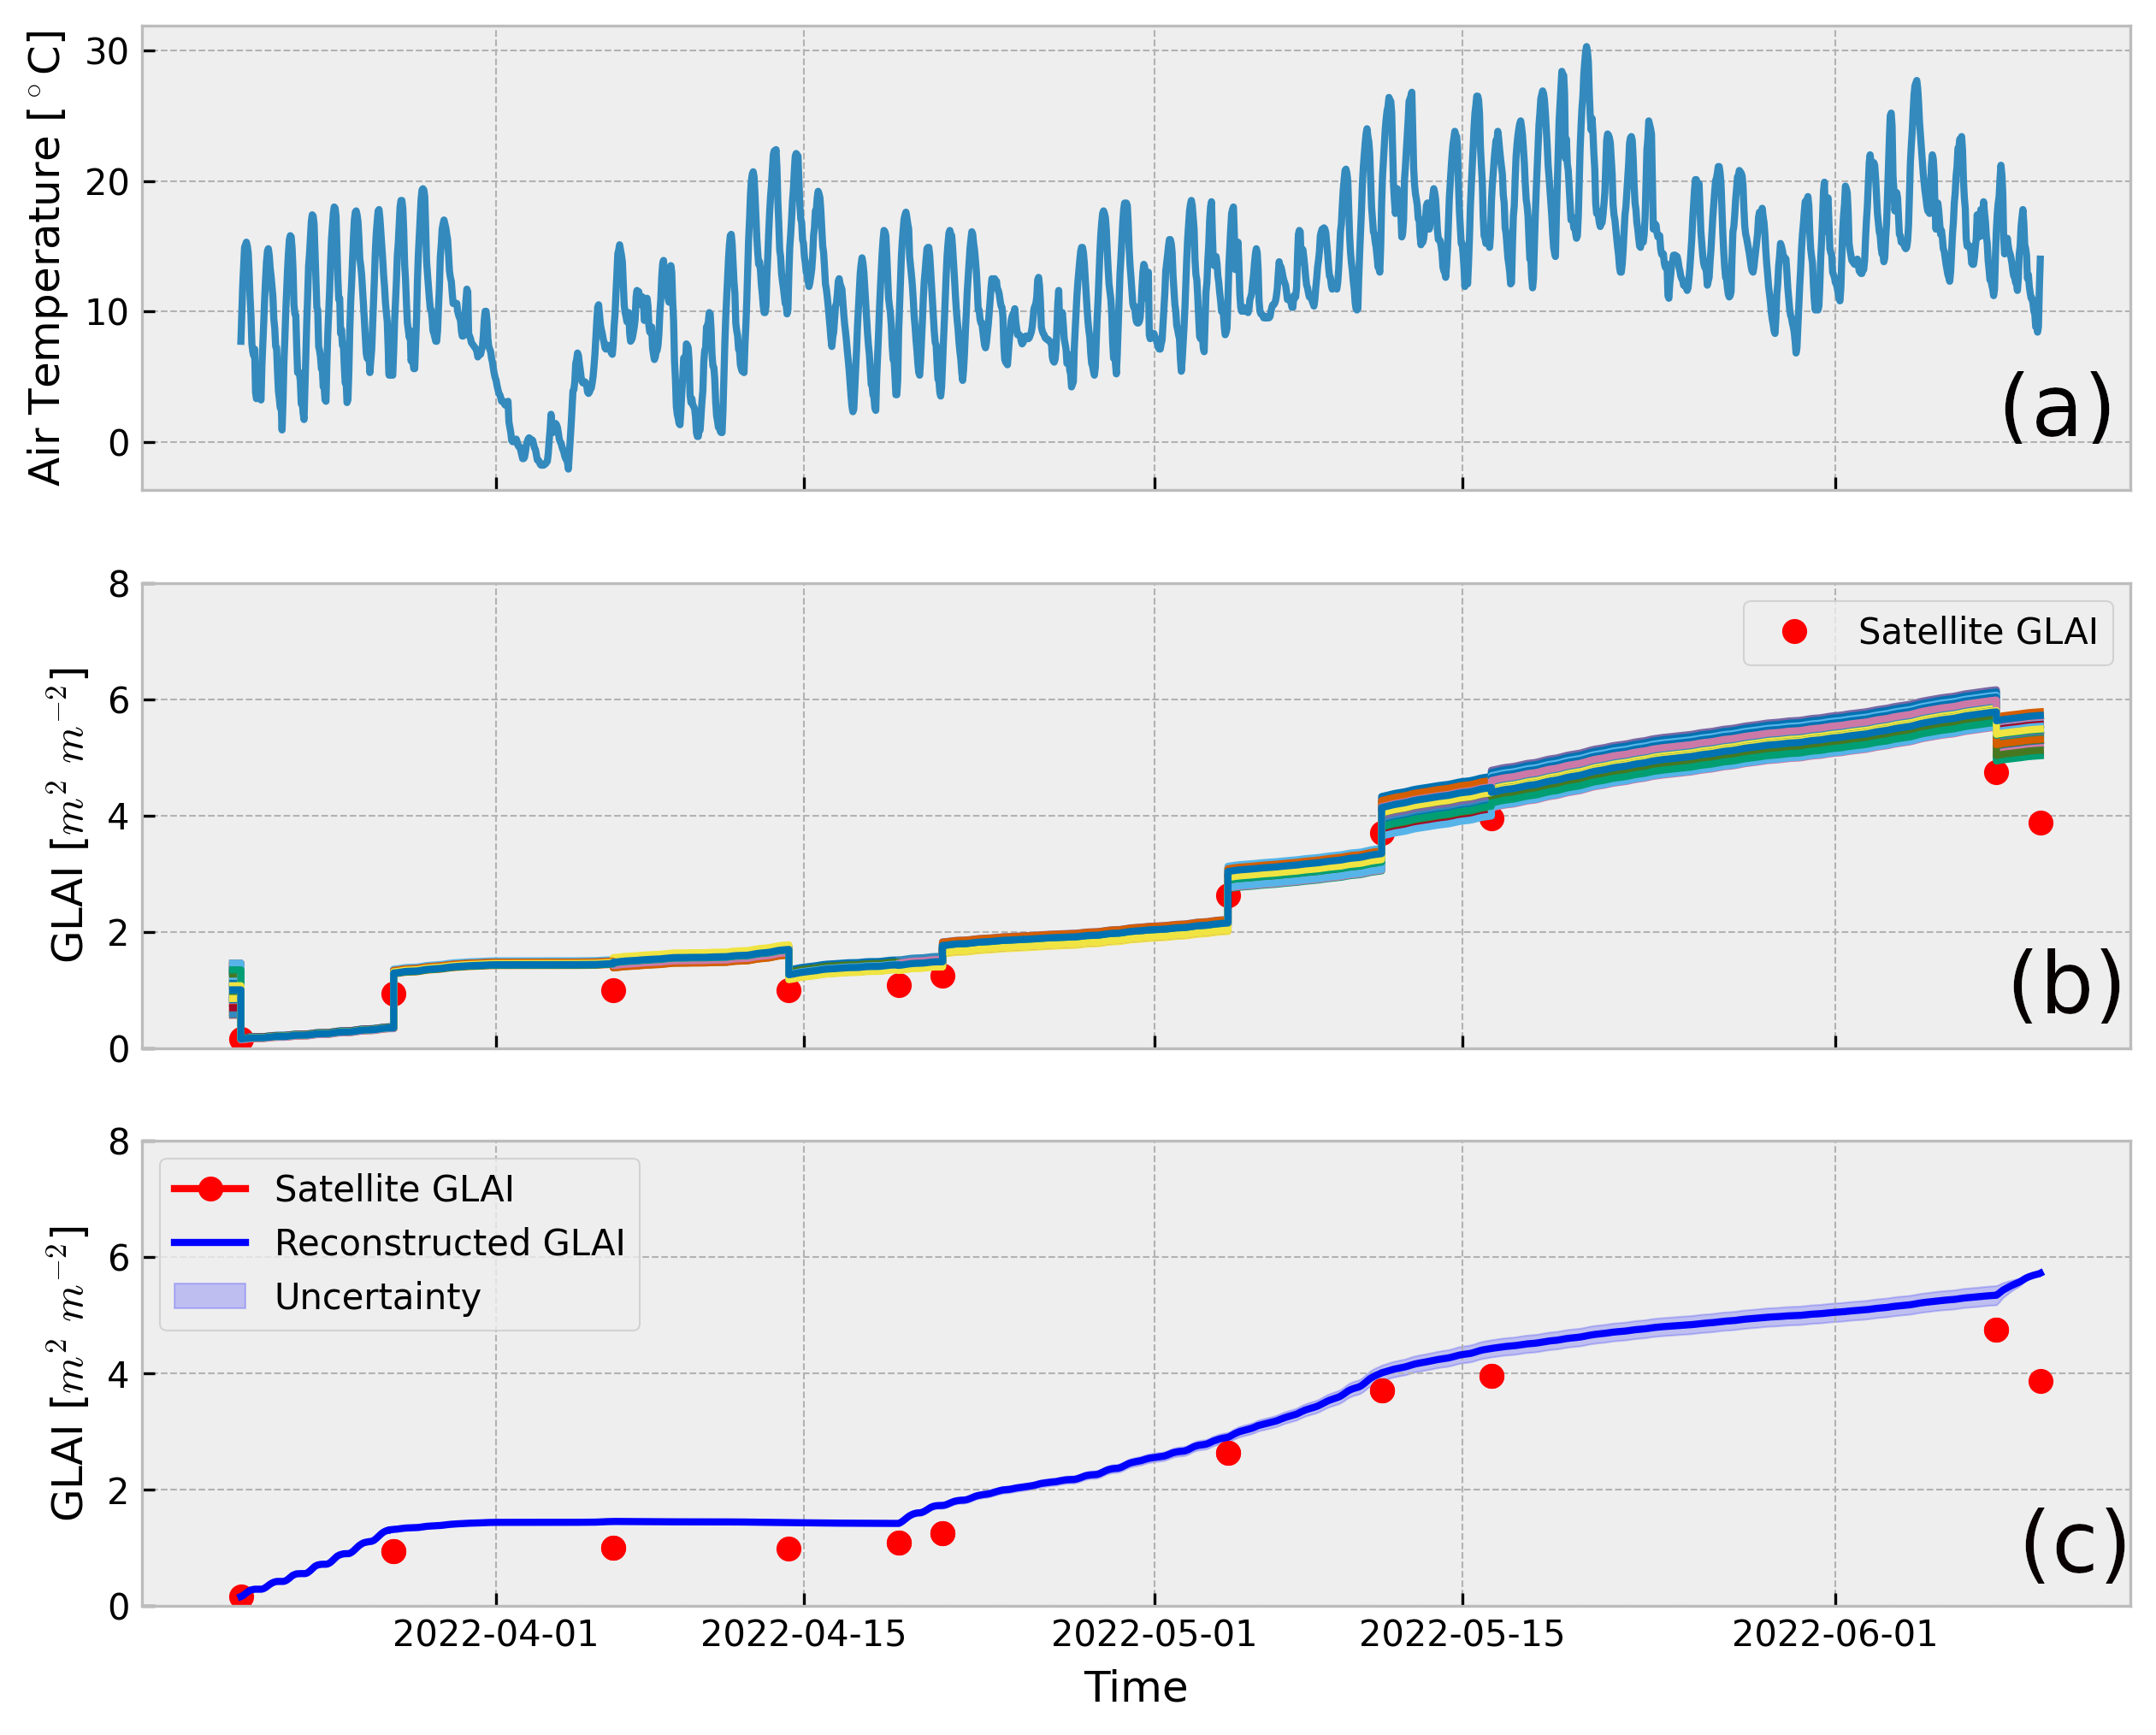
\includegraphics[width=\textwidth]{06-DRC/img/interpolated_lai_5255495.0_475965.0_hourly.png}
    \caption{Example of the proposed probabilistic \gls{GLAI} assimilation for a single \gls{S2} pixel at the Strickhof site in 2022 combining hourly air temperature data (a) with raw \gls{S2} \gls{GLAI} observations (red dots) using \gls{DRC}-based cumulative daily growth rates (solid colored lines in b) to reconstruct \gls{GLAI} time series with associated uncertainties (c). The dose-response curve type used in this case was asymptotic.}
    \label{fig:assimilation-sample-pixel}
\end{figure}

As a first step, we performed a conventional \gls{EnsKF} assimilation (Figure~\ref{fig:assimilation-sample-pixel}b) using \gls{DRC}-based growth rates derived from air temperature time series (Figure~\ref{fig:assimilation-sample-pixel}a). As the \gls{DRC}s provide growth rates, an initial \gls{GLAI} must be provided. We therefore initialised each of the 50 ensembles by randomly sampling between the lower and upper \gls{GLAI} bounds using a uniform probability distribution. The initial \gls{GLAI} bounds were set to a range of 0.5 to 1.5$m^2$ $m^{-2}$ based on empirical knowledge. We started the model runs just before the first \gls{S2} observation (Figure~\ref{fig:assimilation-sample-pixel}b, left). We then accumulated all the \gls{DRC} \gls{GLAI} growth rates up to the first raw \gls{S2} \gls{GLAI} observation. At the time $t$ of the observation, we computed the Kalman gain $K$:

\begin{equation}
\label{eq:kalman-gain}
    K = P_e H^T (H P_e H^T + R_e)^{-1}
\end{equation}
In Equation~\ref{eq:kalman-gain}, $P_e$ and $R_e$ denote the model and observation covariance matrices based on their uncertainties, and $H$ is the measurement operator which is the identity matrix since \gls{GLAI} is directly observable. Using $K$, we calculate the Kalman innovation term $KI$

\begin{equation}
    KI = D - (H A)
\end{equation}
where $D$ denotes the observation matrix with uncertainties and $A$ is the matrix with modelled \gls{GLAI} values at time $t$. Thus, the model state at the analyses step $A^a$ can be obtained:

\begin{equation}
\label{eq:kalman-analyses-step}
    A^a = A + K\ KI
\end{equation}
$A^a$ re-initializes the ensembles at $t$. As before, we then calculated the cumulative \gls{DRC} growth rates until the next raw \gls{S2} \gls{GLAI} observation at time $t+1$. At $t+1$ a new $A^a$ was calculated using Equations~\ref{eq:kalman-gain} to~\ref{eq:kalman-analyses-step}. This procedure was repeated for all \gls{S2} observations except the last one as shown in Figure~\ref{fig:assimilation-sample-pixel}b.

Here, a limitation of the \gls{EnsKF} method becomes clear: \gls{EnsKF} is a non-conservative approach, i.e., potentially large jumps in the modeled time series are caused by the assimilation (Figure~\ref{fig:assimilation-sample-pixel}b). This is physiologically implausible, since GLAI trajectories must be continuous. Therefore, we had to extended the EnsKF approach in a second step:

We addressed said problem by replacing the raw \gls{S2} \gls{GLAI} observations with the ensemble mean at each analysis step $A^a$ ($GLAI_{assim}$). This is to ensure that model and observation information is preserved. The ensemble standard deviation is retained as a measure of uncertainty, taking into account both, model and observation uncertainty. Using the $GLAI_{assim}$ values, we used the \gls{DRC}s for a second time to model growth. This time, however, we used the \gls{DRC}s to interpolate between the $GLAI_{assim}$ values, which are still temporally sparse. We scaled the cumulative growth rates to exactly match the $GLAI_{assim}$ values. In case $GLAI_{{assim}_{t+1}}$ was smaller than $GLAI_{{assim}_{t}}$, $GLAI_{{assim}_{t+1}}$ was discarded. In this case, we interpolated between $GLAI_{{assim}_t}$ and $GLAI_{{assim}_{t+2}}$. This ensured that undetected outliers in the raw \gls{S2} \gls{GLAI} values were not given too much weight, while preserving medium range temporal characteristics. The resulting interpolated \gls{GLAI} curve at the temporal resolution of the \gls{DRC} (i.e., hourly or daily) is shown in Figure~\ref{fig:assimilation-sample-pixel}c, in which the solid blue line denotes the assimilated, \gls{DRC}-interpolated reconstructed \gls{GLAI} time series.

From here on we name the reconstructed time series after the underlying \gls{DRC}s. That is, by "non linear" we mean from now on the \gls{EnsKF} assimilated and interpolated data points created using the non linear \gls{DRC} and raw \gls{S2} \gls{GLAI} observations. The same applies to "asymptotic" and "Wang Engels".

\subsubsection{Baseline method}
\label{subsubsec:baseline-method}
As baseline method, a sigmoid (a.k.a. logistic) function was fitted to the same raw \gls{S2} \gls{GLAI} observations at the pixel scale (Figure~\ref{fig:workflow-glai-time-series}d). Due to its S-shaped form, sigmoid functions are widely used in remote sensing to obtain continuous time series of vegetation traits. The sigmoid function is a simplified version of \gls{DL}~\citep{beck_improved_2006}, which only accounts for the generative (ascending) branch of \gls{GLAI} development. It is therefore a baseline that, unlike other statistical models such as the Savitzky-Golay filter, already has parameters with a certain biological significance.

The sigmoid function takes four parameters: The supremum of the function's values $L$, the growth rate $k$, the function's midpoint $x_0$ and an offset from zero $b$ which is necessary because \gls{GLAI} values around \gls{BBCH} 30 are usually larger than zero:

\begin{equation}
\label{eq:logistic-function}
    f(x) = \frac{L}{1 + e^{-k(x-x_0)}} + b
\end{equation}

A minimum of four raw \gls{S2} \gls{GLAI} observations are required to fit the model parameters. We fit the sigmoid function to each pixel, taking into account all available \gls{GLAI} observations, using the Levenberg-Marquardt algorithm available in the scipy Python library (version 1.11.0) with the function "scipy.optimze.curve\_fit". The maximum number of optimisation steps was set to 1000. The parameterised logistic function (equation~\ref{eq:logistic-function}) was then used to reconstruct the \gls{GLAI} time series at daily resolution. We will refer to this time series as the baseline \gls{GLAI}.

\subsection{Model Validation}

The raw \gls{S2} \gls{GLAI} observations and the reconstructed continuous \gls{DRC} and baseline \gls{GLAI} time series were compared against the independent in-situ validation \gls{GLAI} data (Section~\ref{subsec:validation-data}). We obtained matching tuples of reconstructed and in-situ \gls{GLAI} by time stamp and spatial intersection of the sampling points with the \gls{S2} 10 m pixel grid. In the case of the reconstructed time series (i.e., \gls{DRC} and baseline \gls{GLAI}), each in-situ \gls{GLAI} value could be matched to a modelled \gls{GLAI} value as the time series is continuous and spans the whole time period for which in-situ data was available. For the raw \gls{S2} \gls{GLAI} observations this was not the case due to the aforementioned temporal sparsity of the satellite observations. Therefore, we only used in-situ \gls{GLAI} values that had a satellite overpass with a maximum difference of one day.

Comparison was carried out by means of common error measures of the linear regression between modelled and observed values. Error measures included the \gls{RMSE}, \gls{nRMSE}, \gls{R2}, and bias between reconstructed ($GLAI_{reconstructed}$) and in-situ \gls{GLAI} values ($GLAI_{insitu}$). The bias was calculated using the variance of $GLAI_{reconstructed}$ ($var(GLAI_{reconstructed})$) and the mean of the squared differences ($MSD$) between mean $GLAI_{reconstructed}$, $\mu(GLAI_{reconstructed})$, and $GLAI_{insitu}$ considering all $n$ matching tuples available:

\begin{equation}
    MSD = \frac{1}{n} \sum_{i=0}^{n} (\mu(GLAI_{reconstructed}) - GLAI_{{insitu}_i})^2
\end{equation}
\begin{equation}
    Bias = MSD - var(GLAI_{reconstructed})
\end{equation}

Error statistics were produced for all sites and years as well as for single sites, years and \gls{BBCH} macro stages (i.e, \gls{BBCH} 30-39, 50-59) to assess model performance in space, time, and with respect to phenological development. In addition, we visualized the temporal trajectories of \gls{GLAI} per parcel to evaluate the physiological plausibility and consistency of the reconstructed \gls{GLAI} time series.
